% !TEX TS-program = pdflatex
% !TEX encoding = UTF-8 Unicode

%%% DOCUMENT DEFINITION
\documentclass[11pt, french]{article} % use larger type; default would be 10pt
\usepackage[utf8]{inputenc} % set input encoding (not needed with XeLaTeX)

%%% PAGE DIMENSIONS
\usepackage{geometry} % to change the page dimensions
\geometry{a4paper} % or letterpaper (US) or a5paper or....
\geometry{margin=2cm} % for example, change the margins to 2 inches all round

%%% PACKAGES
\usepackage{graphicx} % support the \includegraphics command and options
\usepackage{booktabs} % for much better looking tables
\usepackage{array} % for better arrays (eg matrices) in maths
\usepackage{paralist} % very flexible & customisable lists (eg. enumerate/itemize, etc.)
\usepackage{verbatim} % adds environment for commenting out blocks of text & for better verbatim
\usepackage{subfig} % make it possible to include more than one captioned figure/table in a single float
\usepackage[frenchb]{babel}

\usepackage{picins,caption}
\usepackage{wrapfig}



%%% HEADERS & FOOTERS
%\usepackage{fancyhdr} % This should be set AFTER setting up the page geometry
%\pagestyle{fancy} % options: empty , plain , fancy

% Rapport projet pluridisciplinaire : etude thermique du pont en H
% : Xavier Galzin, Stanislas Bertrand, Romain Desille, Frédéric Meslin

\title{\textsc{Projet Pluridisciplinaire} \\ Rapport Solution Analogique}
\author{Xavier GALZIN, Stanislas BERTRAND, Romain DESILLE, Frédéric MESLIN}
\date{19/03/2012}

\begin{document}
\maketitle

\pagebreak

\section*{Introduction}
Liste
\\- Rappel des objectifs
\\- liens avec l'étude automatique


%%%%%%%%%%%%%%%%%%%%%%%%%%%%%%%%%%%%%%%%%%%%%%%%%%%%%%%%%%%%%%%%%%%%%%%%%%%%%%%
% Capteur & Conditionnement -> Stan
%%%%%%%%%%%%%%%%%%%%%%%%%%%%%%%%%%%%%%%%%%%%%%%%%%%%%%%%%%%%%%%%%%%%%%%%%%%%%%%


\section{Capteur \& Conditionnement}
\subsection{Capteur à Effet Hall}


\subparagraph*{Principe du capteur à Effet Hall}~\\
\begin{minipage}[t]{10cm}
\vspace{-0.3cm}
\parpic{\includegraphics[width=5cm]{SolutionAnalogique/capteur_effet_hall}}
Un capteur à effet Hall permet de mesurer le champ magnétique $B$ grâce à la déformation d'un courant $I_0$ dans un conducteur ou semi-conducteur, soumis à ce champ. La déformation du flux d'électron génère une différence de potentiels aux bords du conducteur : $V_h =K_h \cdot B \cdot I_0$. Cette relation considère $B$ comme le champ magnétique normal à la surface du conducteur.
\end{minipage}


\subparagraph*{Implantation}~\\
\begin{minipage}[t]{10cm}
Pour mesurer les champs magnétiques de la bobine et du mobile, deux capteurs à effet Hall (modèles Allegro A1302), sont placés à chaque extrémité de la bobine. L'alignement de la bobine, du mobile et des capteurs est important car c'est le champ magnétique normal au capteur qui est mesuré. Il est ainsi possible de connaitre la position verticale du mobile, les deux capteurs étant placés symétriquement sur la bobine, ils mesurent le même champ résultant. Le champ résultant du mobile n'est pas le même pour les deux capteurs, en effet, le champ diminue avec la distance. Le bilan des champs magnétiques exercés sur les capteurs est le suivant :
\vspace{-0.3cm} \[B_{H2} = B_{Bob} + B_{Mob~Dist_{Mob-H2}}\]
\vspace{-0.8cm} \[B_{H1} = B_{Bob} + B_{Mob~Dist_{Mob-H1}}\]
L'image de la position du mobile est contenue dans  $B_{Mob~Dist_{Mob-H2}}$ et $B_{Mob~Dist_{Mob-H1}}$. L'image est obtenue par différence de $B_{H2}$ et $B_{H1}$, $V_{H2}-V_{H1}$
\end{minipage}
~
\begin{minipage}[t]{8cm}
\vspace{-7cm}
\piccaption{Implantation des capteurs}
\parpic{\includegraphics[width=8cm]{SolutionAnalogique/EffetHall}}
\end{minipage}


\subparagraph*{Caractéristiques électronique}~\\
Les capteurs Allegro A1302 conviennent à notre application car ils sont optimisés pour des systèmes de positionnement linéaires ou radiaux. Le capteur peut être alimenté par une tension de 5V, tension utilisé par nos montages analogiques. Le signal de sortie ne nécessite aucun conditionnement car la mesure effectuée est filtrée et amplifiée en interne et le niveau de sortie est directement compatible. Le circuit a une faible impédance de sortie, caractéristique importante pour les montages réalisés par la suite.

\subsection{Montage différentiel}

\begin{wrapfigure}{r}{8cm}
  \includegraphics[width=8cm]{SolutionAnalogique/AmpInst}
  \caption{Amplificateur d'instrumentation}
\end{wrapfigure}
Le montage amplificateur d'instrumentation a été choisi pour son gain différentiel réglable, son taux de réjection en mode commun important grâce à l'étage d'entrée symétrique et ses impédances d'entrées fortes . De plus, ce montage a été spécifiquement développé pour notre type d'applications. D'autres montages soustracteurs plus simples, employant moins d'AOPs, auraient été envisageables mais l'économie de composants réalisée en regard des performances obtenues est discutable pour notre application. 

Un ensemble d'amplificateurs de type LM324 a été employé pour réaliser toutes les fonctions analogiques. Ce boitier a été choisi pour son aptitude à fonctionner en mono-tension, sa bande passante suffisamment élevée pour notre application et son caractère standard impliquant sa disponibilité. Un circuit LM324 comportant 4 AOPs identiques, il est tout indiqué pour l'implantation de l'amplificateur d'instrumentation.

Ce montage n'est pas réalisé de manière complètement intégrée ce qui dégrade ses performances, notamment à cause des imprécisions relatives des résistances $R$. Des composants idoines intégrant toute la structure existent et permettent des mesures de grande précision mais à un prix en rapport direct.

L'étude du schema donne la relation suivante : $V_s=(1+2 \frac{R}{R0})(V_1-V_2) + V_{offset}$. La mesure de la tension maximale de sortie permet de régler la valeur de l'offset, $V_{offset}=\frac{V_{max}}{2}$, $V_{max}=3.7$V. Cela permet de maximiser les variations du signal en le centrant dans la plage de sortie de l'AOP.

\subsection{Consigne Analogique}
\begin{wrapfigure}{r}{0.5\linewidth}
  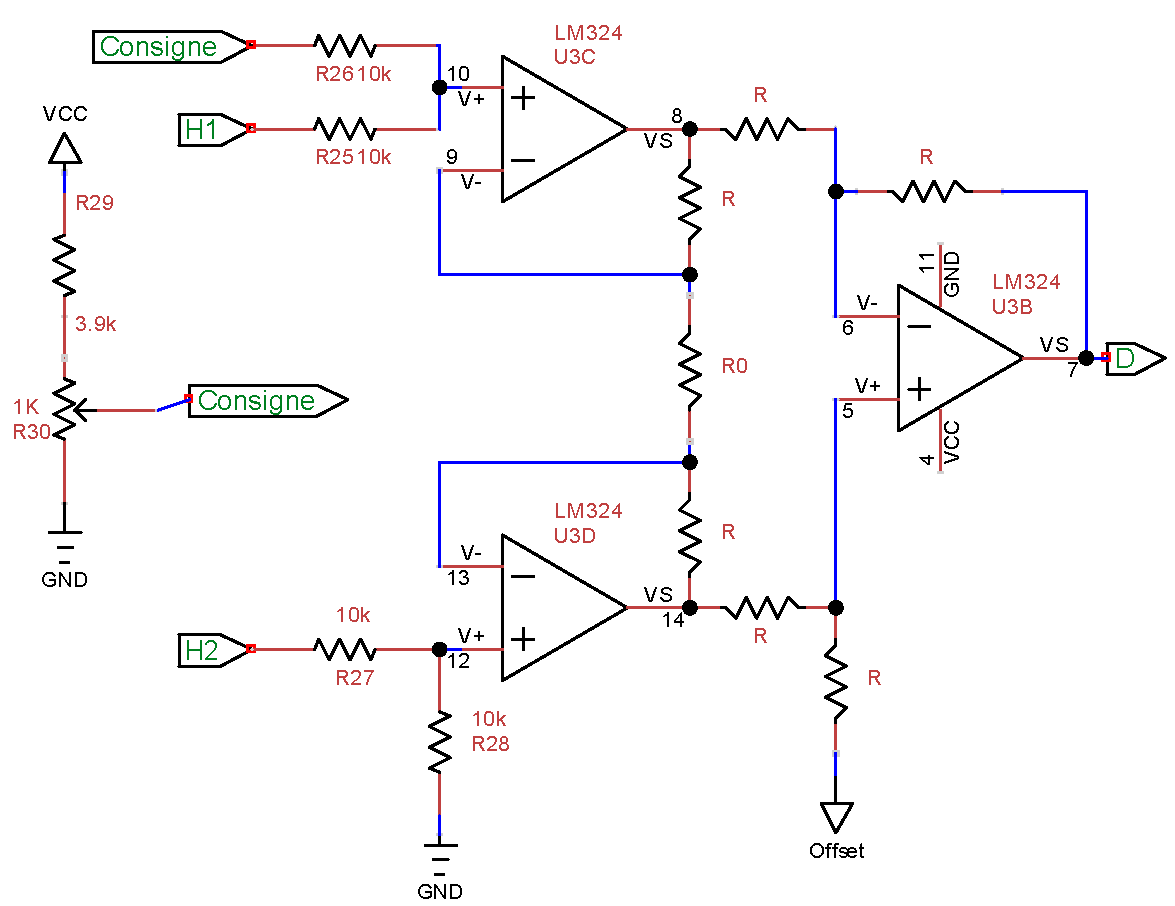
\includegraphics[width=\linewidth]{SolutionAnalogique/AmpInstCons.pdf}
  \label{DiffConsigne}  
  \caption{Différentiel avec consigne}
\end{wrapfigure}
La conception initiale ne prévoyait pas de consigne analogique, seulement une consigne numérique. Il s'est avéré plus intéressant d'ajouter une consigne analogique pour plusieurs raisons : elle permet de générer l'erreur et de travailler centré sur l'offset en sortie du montage différentiel. Cela permet de maximiser la plage du signal pour la numérisation.

La consigne est ajoutée en tirant avantage du montage différentiel. Désormais, sur l'entrée inverseuse du montage, deux signaux sont sommés, la consigne et le capteur $H1$. Le champ magnétique mesuré par $H1$ est plus faible que celui de $H2$ donc $H2-H1>0$. L'ajout de la consigne permet d'annuler cette tension pour une certaine position du mobile (position d'équilibre), la tension de sortie est alors celle de l'offset.
\begin{center}
$V_s=\frac{1}{2}(1+2 \frac{R}{R0})(H2-H1-Consigne) + V_{offset}$
$Consigne = (H2-H1)_{15mm}$
\end{center}
Le sommateur en entrée induit une division par deux des tensions. C'est pourquoi la tension du capteur H2 est également divisée via un pont. Cela est rendu possible grâce à la faible impédance de sortie des capteurs à effet Hall. La génération de consigne respecte cette contrainte, $R_{eq_{Consigne}} \ll R_{26}$. Pour faciliter le réglage, la course du potentiomètre a été fixée de 0 à 1V, ce qui est suffisant pour annuler $H2-H1$. Ce gain d'entrée est compensé par le gain du montage différentiel. 


%%%%%%%%%%%%%%%%%%%%%%%%%%%%%%%%%%%%%%%%%%%%%%%%%%%%%%%%%%%%%%%%%%%%%%%%%%%%%%%
% Correcteur Avance de phase
%%%%%%%%%%%%%%%%%%%%%%%%%%%%%%%%%%%%%%%%%%%%%%%%%%%%%%%%%%%%%%%%%%%%%%%%%%%%%%%


\section{Correcteur Avance de phase}

Liste
\\- Choix du montage
\\- Choix dex couples R-C ( Cf Meca ) ( Choix des série E6, E12 et du type des condensateurs)
\\- Etude du gain du montage


\subsection{Données}

\noindent
Pour le schémas et les formules (que nous avons quand même vérifié) du correcteur, nous nous sommes servi d'un schémas trouvé sur internet (voir Bibliographie) :

\begin{center}
\includegraphics[width = 15cm]{SolutionAnalogique/Avph.png} 
\end{center}

\vspace{0.5cm}

Dans ce schémas, le produit $R_1*C_1$ correspond à la constante $ T_av$ définie dans le rapport d'automatique et le produit $R_2*C_2$ correspond à $0.1*T_av$.


Nous allons déterminer les valeurs de $R_1$, $R_2$, $C_1$ et $C_2$ dans deux configurations : poids du mobile à $0.0897 kg$ correspondant à un $T_av$ de 0.0313 et poids du mobile à $0.1414 kg$ correspondant à un $T_av$ de 0.0393.


Aussi, par le biais de MATLAB, nous avons pu obtenir la courbe théorique de notre correcteur par avance de phase :

\begin{center}
\includegraphics[width = 15cm]{SolutionAnalogique/aphmat.png} 
\end{center}

A noter que la fréquence donnée est en $rad.s^-1$, elle vaut environ 16Hz. 
\subsection{Détermination de valeurs des composants}

Pour des raisons de simplifications, nous prendrons les résistances $R_1$ et $R_2$ égales, le facteur 10 entre les constantes du numérateur et du dénominateur sera donc réalisé par un facteur 10 entre les valeurs des condensateurs. 



Pour le poids de $0.0897 kg$, en choisissant des composants avec des valeurs normalisées, on obtient $R=8.2 K\Omega$, $C_1=3.9 \mu F$ et $C_2=390 nF$. 



On fera plutôt varier les résistances que les condensateurs pour s'adapter au changement de poids. On conserve donc les mêmes valeurs de condensateurs. On trouve alors $R=10.076 K\Omega$. 



Il sera donc possible de prendre des potentiomètres pour ajuster les constantes, corrigeant ainsi les écards possibles des valeurs de condensateurs. 


\subsection{Validation par simulation PSpice}

On simule le correcteur à avance de phase par le schémas suivant : 

\begin{center}
\includegraphics[width = 15cm]{SolutionAnalogique/schAvph.png} 
\end{center}

On obtient le résultat de simulation suivant : 

\begin{center}
\includegraphics[width = 15cm]{SolutionAnalogique/simuAvph.png} 
\end{center}

Comme on peut le voir en comparant par rapport au résultat donné par MATLAB, le schéma répond comme on le souhaitait. 

\vspace{0.5cm}
\subsection{Conclusion}

\noindent
Nous avons donc validé notre choix de montage de correcteur et nous avons déterminer des valeurs admissibles de composants analogiques grâce à cette étude. Il faudra cependant être attentif quant au choix des condensateurs vis-à-vis de leur fréquence de fonctionnement.  

\subsection{Bibliographie}

- Cours de GEE, A. Meghebbar :
\newline \textit{\underline{fsi.univ-tlemcen.dz/cours/Support-Cours-Commande-Analogique-Master-Electrotechnique10.pdf}}


\section{Conversion \& Comunication}
\subsection{Choix du microcontrolleur}
Liste
\\- Tension d'alimentation
\\- Frequence de travail
\\- module de conversion
\\- Disponibilité des outils de dev
\\- instructions evoluées MUL \& DIV pour le correcteur numérique

\subsection{Conversion A/D - PWM}
Liste
\\- Utilisation des modules
\\- Programme + Explications

\subsection{Communication serie/USB}
Liste
\\- Ajout d'un driver USB/Série
\\ Programme le cas échéant

\section{Control de puissance}
Liste
\\- choix du pont complet ( Justification )
\\-  - Attraction | Répulsion de la bobine
\\-  - Asservissement à l'équilibre ?
\\- Choix du composant
\\- Réalisation PCB
\\-  - Problème thermique
\\-  - Problème de boitier
\\- Utilisation du four à réfusion

\subsection{Données}

\noindent
D'après la Datasheet du A4950 :

\vspace{0.5cm}

\noindent
$ 
R_{TH} = 62 \char123C/W  \\
T_{JUNC\_MAX} = 160 \char123C  \\
T_{AMB} = 25\char123C  \\
R_{DSON} = 1.3 \Omega  \\
$



\noindent
A noter que cette valeur de $R_{TH}$ est donnée dans le cas l'on a aurait des plages de cuivres d'environ 2cm par 2cm de chaque côté du composant. De plus, la valeur de $R_{DSON}$ est une valeur pire cas.

\subsection{Equations}

\noindent
L'équation de la température de la jonction est donnée par :

\vspace{0.5cm}

\noindent
$
T_{JUNC} = R_{TH} * P_{DIS} + T_{AMB}
$

\vspace{0.5cm}

\noindent
P étant la puissance \textbf{dissipée} dans le composant que l'on calculera par la formule :

\vspace{0.5cm}

\noindent
$
P_{DIS} = R_{DSON} * I\up{2} = 1.3 * 1.28\up{2} = 5.2 W
$

\vspace{0.5cm}

\noindent
Finalement, on obtient :

\vspace{0.5cm}

\noindent
$
T_{JUNC} = 62 * 5.2 + 25 = 157.06 \char123 C
$

\subsection{Conclusion}

\noindent
Le résultat trouvé est très proche de la valeur limite du composant. Cependant, nous avons pris des paramètres extrèmes qui ne seront normalent pas atteint. De plus, nous comptons augmenter la surface de cuivre qui assurera la dissipation afin d'obtenir une marge plus grande par rapport à ce résultat.

\section{Résultats - Evolution}
Liste
\\- Monitoring du fonctionnement
\\- Résulatat expérience
\\- Ouverture vers correcteur numérique

\subsection{Protocole de Test / Mise en fonctionnement ?}

Liste
\\- Règlage du différentiel ( Consigne et Gain )
\\- Vérification de l'avance de phase ( rq : le montage n'a pas d'inverseur )
\\- numérisation et génération PWM ( Fonction de transfere )
\\- vérification du comportement globale ( Fonction de transfere )


\end{document}
